\documentclass[a4paper, 12pt]{article}

\usepackage[UTF-8]{ctex}
\usepackage{indentfirst}
\usepackage{amsmath}
\usepackage{tabularray}
\usepackage{xcolor}
\usepackage{listings}
\usepackage{subfigure}
\usepackage[graphicx]{realboxes}

\lstset{
    basicstyle          =   \sffamily,
    keywordstyle        =   \bfseries,
    commentstyle        =   \rmfamily\itshape,
    stringstyle         =   \ttfamily,
    flexiblecolumns,
    numbers             =   left,
    showspaces          =   false,
    numberstyle         =   \zihao{-5}\ttfamily,
    showstringspaces    =   false,
    captionpos          =   t,
    frame               =   lrtb,
}

\lstdefinestyle{Python}{
    language        =   Python,
    basicstyle      =   \zihao{-5}\ttfamily,
    numberstyle     =   \zihao{-5}\ttfamily,
    keywordstyle    =   \color{blue},
    keywordstyle    =   [2] \color{teal},
    stringstyle     =   \color{magenta},
    commentstyle    =   \color{red}\ttfamily,
    breaklines      =   true,
    columns         =   fixed,
    basewidth       =   0.5em,
}

\setlength{\parindent}{2em}
\numberwithin{equation}{section}

\begin{document}

    \title{基于''XXX''的低碳建筑研究}
    \author{}
    \date{}
    \maketitle

    \centerline{\textbf{\LARGE{摘要}}}

    \textbf{\large{关键词}}

    {\centering{\section{问题重述}}}
        \subsection{问题背景}
        “双碳”即碳达峰与碳中和的简称,我国力争2030年前实现碳达峰,2060年前实现碳中和。
        “双碳”战略倡导绿色、环保、低碳的生活方式。我国加快降低碳排放步伐,大力推进绿色低碳科技创新,以提高产业和经济的全球竞争力。
        低碳建筑是指在建筑材料与设备制造、施工建造和建筑物使用的整个生命周期内,减少化石能源的使用,提高能效,降低二氧化碳排放量。

        \subsection{目标任务}
            \textbf{问题一:}计算给定建筑通过空调调节温度的年碳排放量。

            \textbf{问题二:}建立综合评价模型,找出易于量化的指标,评估居住建筑整个生命周期的碳排放。

            \textbf{问题三:}基于问题二,考虑建筑生命周期三个阶段的碳排放问题,对江苏省13个地级市的居住建筑进行评价,验证模型的有效性。

            \textbf{问题四:}建立碳排放预测模型,基于江苏省建筑全过程碳排放的历史数据,对2023年江苏省建筑全过程的碳排放量进行预测。

            \textbf{问题五:}结合前面的讨论给出江苏省建筑碳减排的政策建议。


    {\centering{\section{问题分析}}}
        \subsection{问题一}
            问题一要求计算通过空题调节温度产生的年碳排放量。
            我们需先求出空调制热和制冷的热量,借此通过\textit{COP}和\textit{EER}求出空调消耗的电量,最后转换成碳排放。
            其中\textit{COP}和\textit{EER}的定义分别为
            \begin{equation}
                COP = \frac{Q_{heat}}{W},\hspace{2em} EER = \frac{Q_{cold}}{W}
            \end{equation}
            $ Q_{heat} / Q_{cold} $指的是单位时间内的制热/制冷量,单位为\textit{J},
            公式中\textit{W}指的是单位为时间内空调消耗的功率,单位为\textit{W}

            首先计算出建筑物各个月的能量需求量。设室内温度要维持的温度为 $ t_{in} $,室外温度为 $ t_{out} $,
            当月该地区平均温度为 $ t_{ave} $ ,方便起见,我们规定
            \begin{equation*}
                t_{out} = t_{ave}
            \end{equation*}
            \begin{equation*}
                t_{in} =
                \begin{cases}
                    18 ^{\circ}C & \text{ $ t_{out} < 18 ^{\circ}C $ } \\
                    t_{out} & \text{ $ t_{out} \in [18 ^{\circ}C, 26 ^{\circ}C] $ } \\
                    26 ^{\circ}C & \text{ $ t_{out} > 26 ^{\circ}C $}
                \end{cases}
            \end{equation*}

            我们使用热传导方程计算用来需要制热/制冷的热量,其形式为
            \begin{equation}
                \Phi = \frac{\lambda \cdot A \cdot |\Delta T|}{\delta}
            \end{equation}
            其中$ \Phi $表示传热速率,$ \lambda $为导热系数,\textit{A}为传热面积,
            $ \Delta T $是室内外温度差,即$ t_{in} - t_{out} $,$ \delta $表示材料厚度。

            将建筑分成墙、门窗、房顶、地面四个部分,分别计算并累加即可得到需要制热/制冷的热量,设为$ Q_{make} $,
            由\textit{COP}和\textit{EER}的定义可得到需电量$ Q_{elec} $和热量$ Q_{make} $的转化关系
            \begin{equation}
                Q_{elec} =
                \begin{cases}
                    \frac{Q_{make}}{EER} & \text{ $ \Delta t < 0 $ } \\
                    0 & \text{ $ \Delta t = 0 $ } \\
                    \frac{Q_{make}}{COP} & \text{ $ \Delta t > 0 $ }
                \end{cases}
            \end{equation}

            最后根据需电量与碳排放的换算关系 $ m = Q_{elec} \cdot 0.28 $ 求出每月碳排放后累加,即得到年度碳排放量。


    {\centering{\section{模型假设}}}


    {\centering{\section{符号说明}}}


    {\centering{\section{模型的建立与求解}}}
        \subsection{问题一的模型建立与求解}

        \subsection{问题二的模型建立与求解}
            \subsubsection{建立层次结构模型}
                \begin{figure}
                    \centering
                    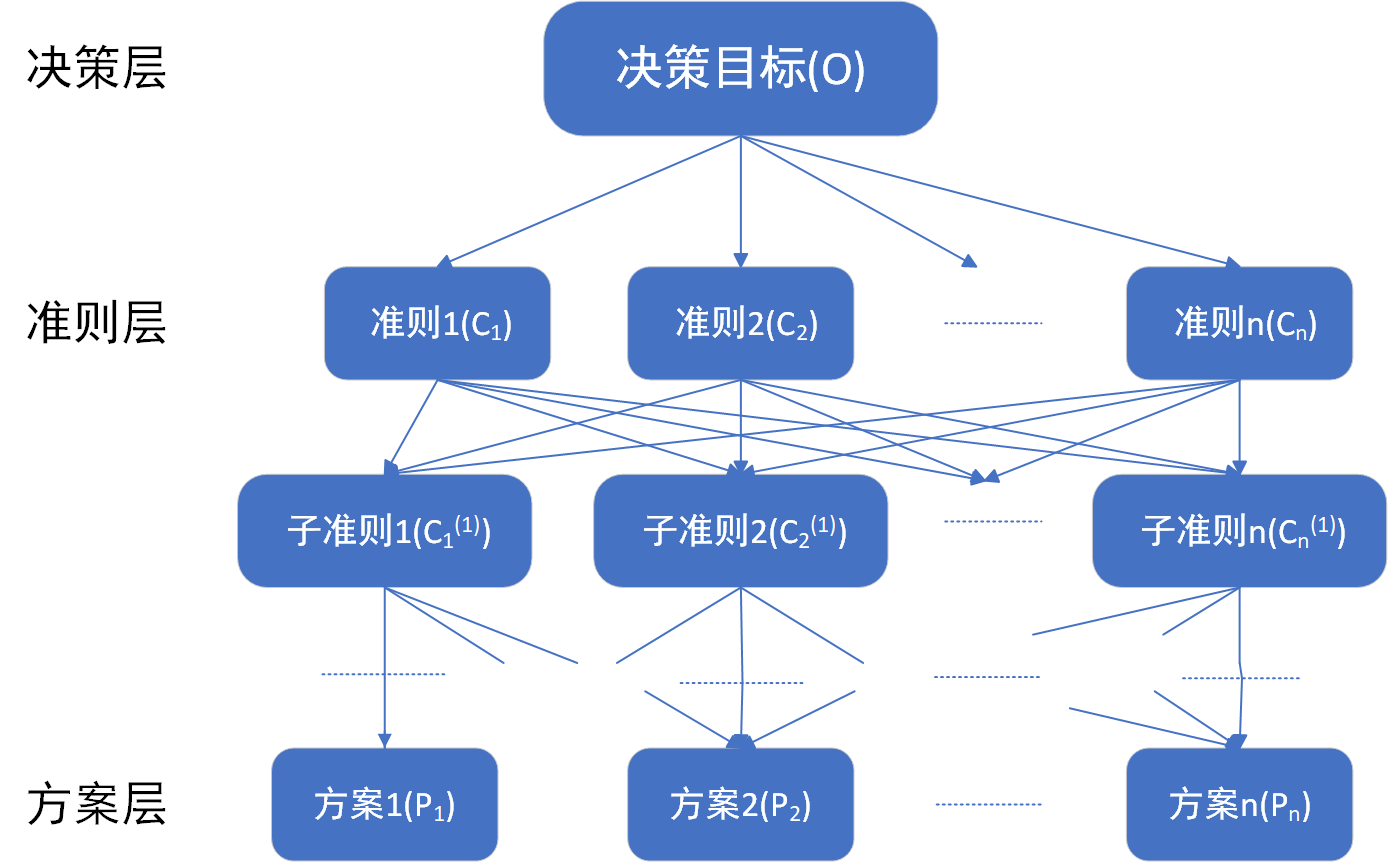
\includegraphics[height=4.5cm,width=9.5cm]{层次分析法框架.png}
                    \caption{层次分析法框架}
                \end{figure}

    {\centering{\section{结果检验与误差分析}}}


    {\centering{\section{模型评价}}}


    {\centering{\section{模型推广与改进}}}


    {\centering{\section{参考文献}}}
    \newpage


    {\centering{\section{附录}}}
        \subsection*{附录A \hspace{2em} 问题一}
            \lstinputlisting[
                style       =   Python,
                caption     =   {\bf Question1},
                label       =   {Question1.py}
            ]{Question1.py}

        \subsection*{附录B \hspace{2em} 问题二}
            \lstinputlisting[
                style       =   Python,
                caption     =   {\bf Question2},
                label       =   {Question2.py}
            ]{Question2.py}

        \subsection*{附录C \hspace{2em} 问题三}

        \subsection*{附录D \hspace{2em} 问题四}

        \subsection*{附录E \hspace{2em} 问题五}

\end{document}
